\documentclass{article}

\usepackage{graphicx}
\usepackage{tikz}
\usepackage{tikzsymbols}
\usetikzlibrary{calc,patterns,shapes.geometric}
\pagestyle{empty}
\usepackage[margin=0pt]{geometry}
\geometry{papersize={14in,12in}}

\def\centerarc[#1](#2)(#3:#4:#5){\draw[#1] ($(#2)+({#5*cos(#3)},{#5*sin(#3)})$) arc (#3:#4:#5);}

\begin{document}
	\begin{figure}
		\centering
		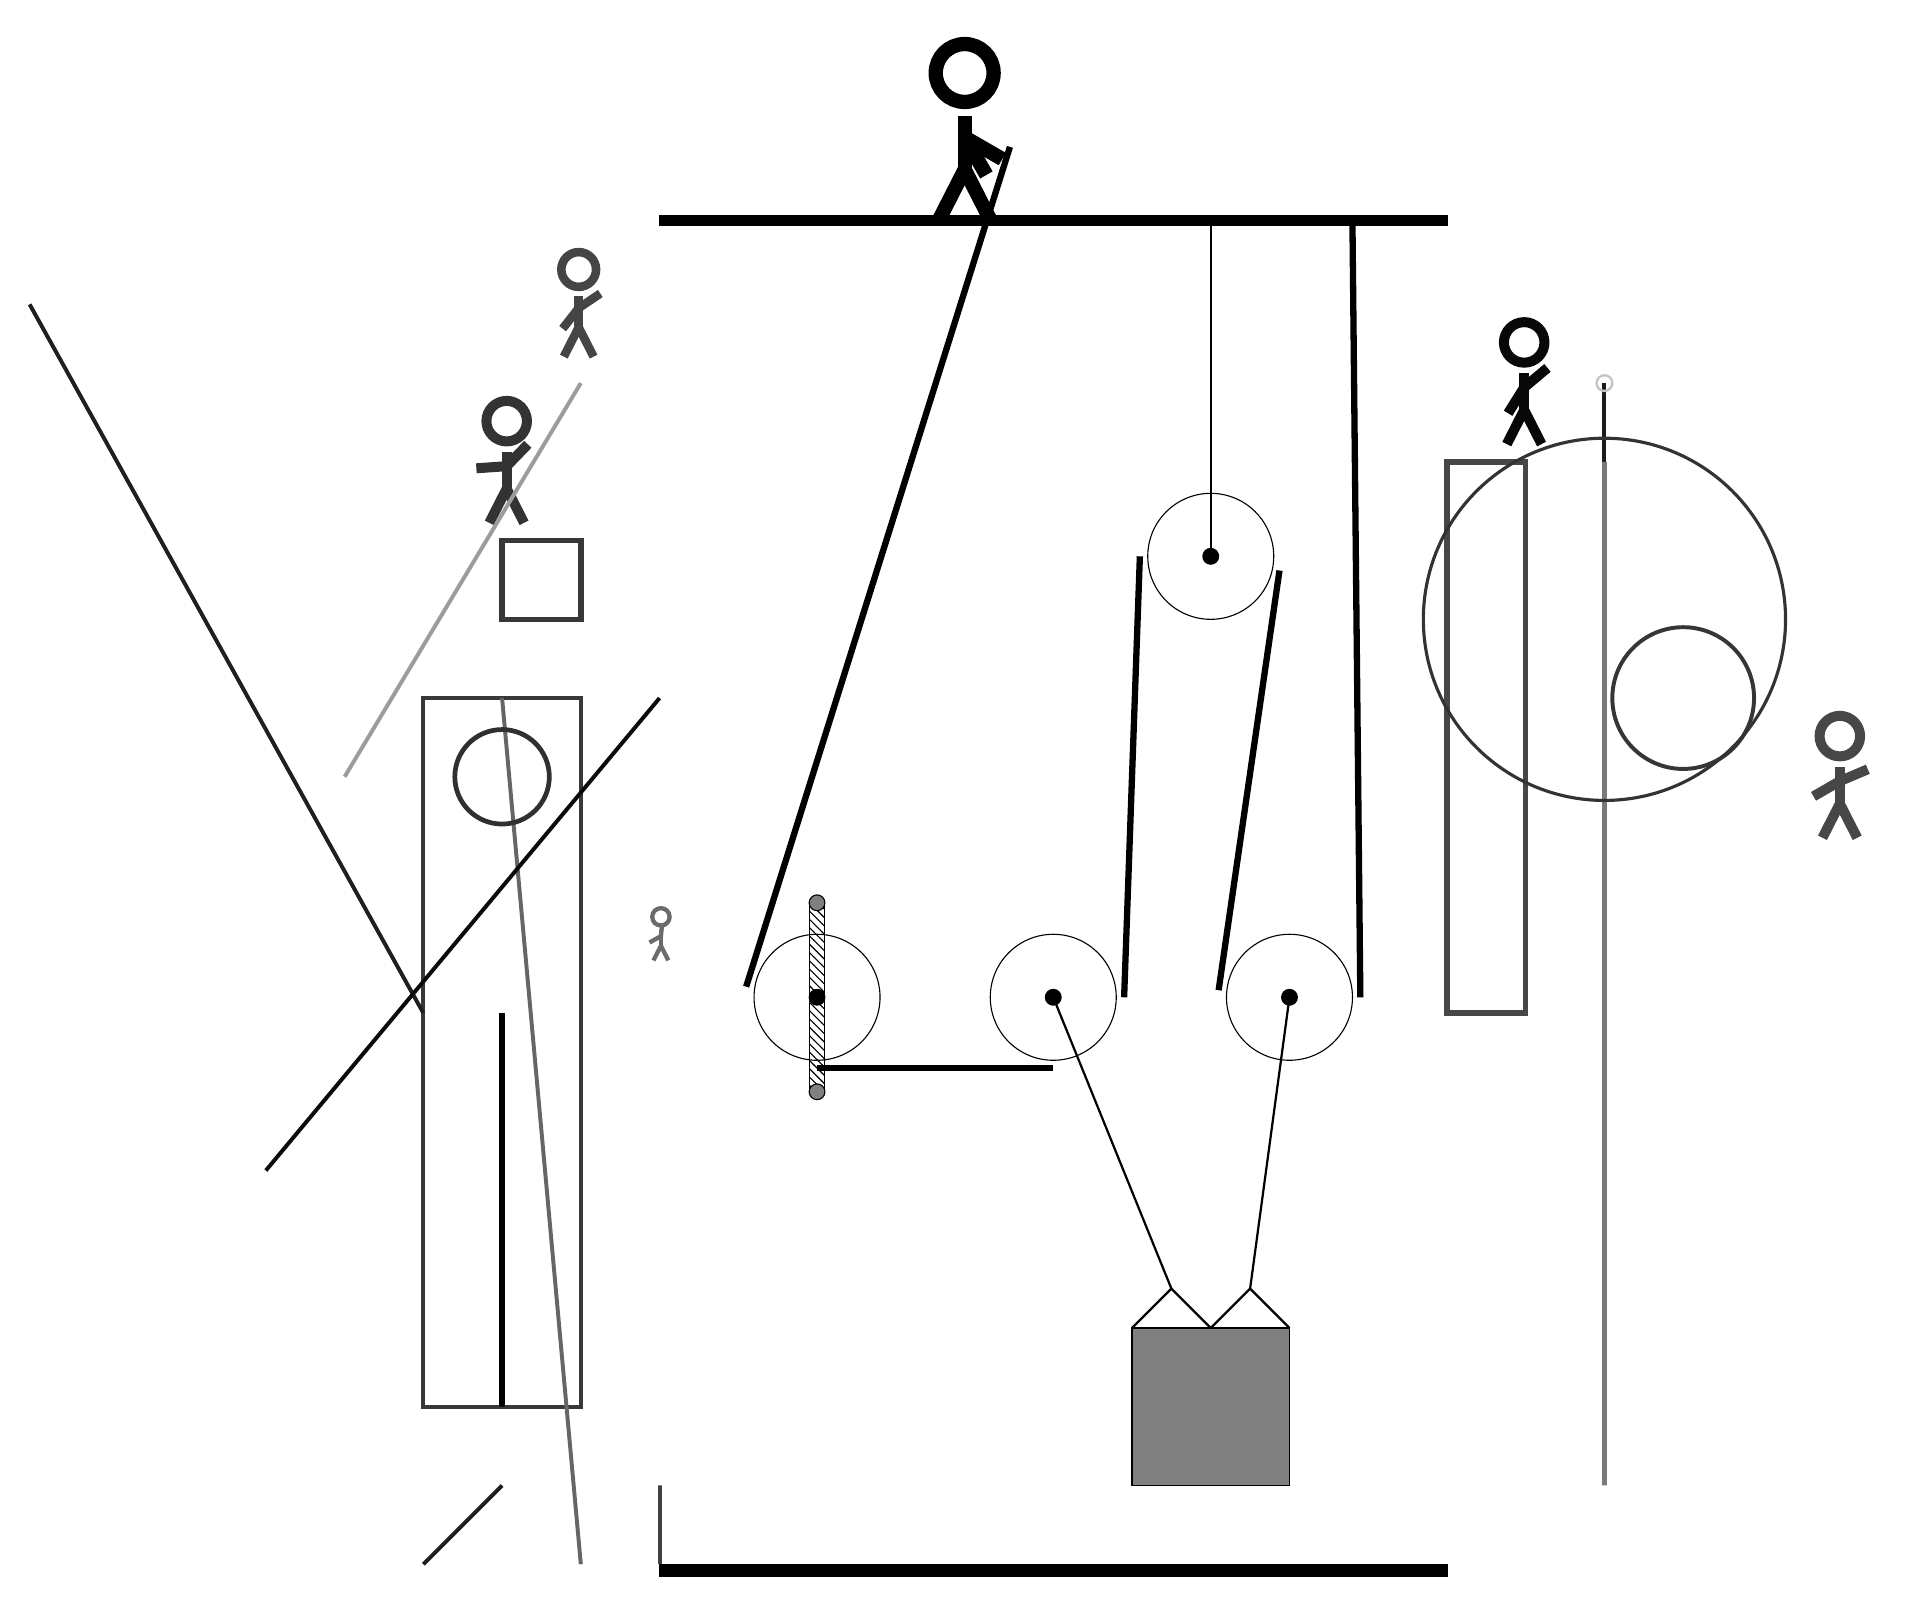
\begin{tikzpicture}
			%%%%% START %%%%%
			
			\draw[fill=black] (-4, 14) rectangle (6, 14.125);
			
			\draw (1, 4.2) circle (0.8);
			\draw[fill=black] (1, 4.2) circle (0.1);
			
			\draw (3, 9.8) circle (0.8);
			\draw[fill=black] (3, 9.8) circle (0.1);
			\draw[thick] (3, 9.8) -- (3, 14);
			
			\node[line width=0.3mm, color=black!97] at (7, 12) {\Strichmaxerl[7][58][40]};
			
			\node[line width=0.6mm, color=black!80] at (-6, 11) {\Strichmaxerl[7][4][46]};
			\node[line width=0.2mm, color=black!58] at (-4, 5) {\Strichmaxerl[3][29][84]};
			\node[line width=0.2mm, color=black!73] at (-5, 13) {\Strichmaxerl[6][52][34]};
			\draw[line width=0.7mm, color=black!78] (-5, 10) rectangle (-6, 9);
			\draw[line width=0.5mm, color=black!78] (-5, -1) rectangle (-7, 8);
			
			\draw[line width=0.5mm, color=black!60](-6, 8) -- (-5, -3);
			\draw[line width=0.5mm, color=black!89](8, 9) -- (8, 12);
			\draw[line width=0.5mm, color=black!88](-7, 4) -- (-12, 13);
			\draw[line width=0.5mm, color=black!24] (8, 7) rectangle (8, -1);
			\draw[line width=0.7mm, color=black!72] (6, 11) rectangle (7, 4);
			\draw[line width=0.7mm, color=black!100] (-6, -1) rectangle (-6, 4);
			\draw[line width=0.5mm, color=black!96](-4, 8) -- (-9, 2);
			
			\draw[line width=0.5mm, color=black!88](-6, -2) -- (-7, -3);
			\draw[line width=0.7mm, color=black!52] (8, -2) rectangle (8, 11);
			\draw [line width=0.5mm, color=black!79](9, 8) circle (0.9);
			
			\node[line width=0.2mm, color=black!72] at (11, 7) {\Strichmaxerl[7][30][23]};
			\draw [line width=0.3mm, color=black!23](8, 12) circle (0.1);
			\draw[line width=0.5mm, color=black!39](-5, 12) -- (-8, 7);
			\draw [line width=0.4mm, color=black!80](8, 9) circle (2.3);
			\draw[line width=0.5mm, color=black!74] (-4, -3) rectangle (-4, -2);
			
			\draw [line width=0.6mm, color=black!81](-6, 7) circle (0.6);
			
			
			\draw (4, 4.2) circle (0.8);
			\draw[fill=black] (4, 4.2) circle (0.1);
			
			\draw[thick] (4, 4.2) -- (3.5, 0.5);
			\draw[thick] (1, 4.2) -- (2.5, 0.5);
			\draw[thick]  (2, 0) -- (2.5, 0.5) -- (3, 0);
			\draw[thick]  (3, 0) -- (3.5, 0.5) -- (4, 0);
			\draw[fill=black!50] (2, 0) rectangle (4, -2);
			
			\draw (-2, 4.2) circle (0.8);
			\draw[fill=black] (-2, 4.2) circle (0.1);
			\draw[pattern=north west lines, pattern color=black] (-2.1, 5.4) rectangle (-1.9, 3.0);
			\draw[fill=black!50] (-2, 5.4) circle (0.1);
			\draw[fill=black!50] (-2, 3.0) circle (0.1);
			
			\draw[line width=0.8mm] (0.45, 15) -- (-2.9, 4.335);
			\centerarc[line width=0.8mm](-2, 4.2)(160:270:0.9);
			\draw[line width=0.8mm](-2, 3.3) -- (1, 3.3);
			\centerarc[line width=0.8mm](1, 4.2)(270:360:0.9);
			\draw[line width=0.8mm] (1.9, 4.2) -- (2.1, 9.8);
			\centerarc[line width=0.8mm](3, 9.8)(-20:180:0.9);
			\draw[line width=0.8mm](3.873, 9.62) -- (3.1, 4.29);
			\centerarc[line width=0.8mm](4, 4.2)(160:360:0.9);
			\draw[line width=0.8mm](4.9, 4.2) -- (4.8, 14);
			
			\node at (-0.07, 15.2) {\Strichmaxerl[10][120][-30]};
			
			\draw[fill=black] (-4, -3) rectangle (6, -3.15);
			
			%%%%% END %%%%%
		\end{tikzpicture}
	\end{figure}	
\end{document}